\documentclass[../../../interview-questions.tex]{subfiles}

\begin{document}

\subsection{Synchronized锁优化}

早期,Synchronized属于重量级锁(Heavyweight Lock),效率低下,因为早期的重量级锁是依赖于底层的操作系统的Mutex Lock来实现的,Mutex Lock在没有获取到锁的情况下直接挂起,而这个挂起是比较消耗资源的,CPU要保存当前线程的执行状态,后面还需要唤醒挂起的线程,而操作系统实现线程之间的切换时需要从用户态(User Model)转换到核心态(Kernel Model)\footnote{从用户态到内核态切换过程中,Linux主要做的事:

1:读取tr寄存器,访问TSS段

2:从TSS段中的sp0获取进程内核栈的栈顶指针

3:  由控制单元在内核栈中保存当前eflags,cs,ss,eip,esp寄存器的值。

4:由SAVE\_ALL保存其寄存器的值到内核栈

5:把内核代码选择符写入CS寄存器,内核栈指针写入ESP寄存器,把内核入口点的线性地址写入EIP寄存器},这个状态之间的转换需要相对比较长的时间\footnote{\url{https://www.cnblogs.com/justcxtoworld/p/3155741.html}},时间成本相对较高,这也是为什么早期的synchronized效率低的原因。庆幸的是在Java 6之后Java官方对从JVM层面对synchronized较大优化,所以现在的synchronized锁效率也优化得很不错了,Java 6之后,为了减少获得锁和释放锁所带来的性能消耗(阻塞或唤醒一个Java线程需要操作系统切换CPU状态来完成,这种状态转换需要耗费处理器时间。如果同步代码块中的内容过于简单,状态转换消耗的时间有可能比用户代码执行的时间还要长),引入了偏向锁(Biased Lock)、轻量级锁(Lightweight Lock)和自旋锁(Spin Lock)等概念,接下来我们将简单了解一下Java官方在JVM层面对Synchronized锁的优化。优化后的流程为:

\begin{itemize}
    \item {首先,synchronized 会尝试使用偏向锁的方式去竞争锁资源,如果能够竞争到偏向锁,表示加锁成功直接返回。}对应的Hotspot C++实现代码:
    
\begin{lstlisting}[language=C++]
void ObjectSynchronizer::fast_enter(Handle obj, BasicLock* lock,
                                    bool attempt_rebias, TRAPS) {
  if (UseBiasedLocking) {
    if (!SafepointSynchronize::is_at_safepoint()) {
      BiasedLocking::Condition cond = BiasedLocking::revoke_and_rebias(obj, attempt_rebias, THREAD);
      if (cond == BiasedLocking::BIAS_REVOKED_AND_REBIASED) {
        return;
      }
    } else {
      assert(!attempt_rebias, "can not rebias toward VM thread");
      BiasedLocking::revoke_at_safepoint(obj);
    }
    assert(!obj->mark()->has_bias_pattern(), "biases should be revoked by now");
  }

  slow_enter(obj, lock, THREAD);
}
\end{lstlisting}


    \item {如果竞争锁失败,说明当前锁已经偏向了其他线程。需要将锁升级到轻量级锁,在轻量级锁状态下,竞争锁的线程根据自适应自旋次数去尝试抢占锁资源。}
    \item {如果在轻量级锁状态下还是没有竞争到锁,就只能升级到重量级锁。在重量级锁状态下,没有竞争到锁的线程就会被阻塞。处于锁等待状态的线程需要等待获得锁的线程来触发唤醒。}
\end{itemize}

锁升级有一个问题,就是没有提到哪里自旋,偏向锁、轻量级锁、重量级锁都没有提到哪里有自旋。自旋是在已经升级成重量级锁之后,线程如果没有争抢到锁,会进行一段自旋等待锁的释放。代码在JDK的objectMonitor.cpp中,获取锁失败,等待锁的释放时使用EnterI()方法:

\begin{lstlisting}[language=C++]
void ObjectMonitor::EnterI(TRAPS) {
    Thread * const Self = THREAD;
    assert(Self->is_Java_thread(), "invariant");
    assert(((JavaThread *) Self)->thread_state() == _thread_blocked, "invariant");
    
    // Try the lock - TATAS
    if (TryLock (Self) > 0) {
        assert(_succ != Self, "invariant");
        assert(_owner == Self, "invariant");
        assert(_Responsible != Self, "invariant");
        return;
    }
    
    DeferredInitialize();
    
    if (TrySpin (Self) > 0) {
        assert(_owner == Self, "invariant");
        assert(_succ != Self, "invariant");
        assert(_Responsible != Self, "invariant");
        return;
    }
}      
\end{lstlisting}

\paragraph{偏向锁(Biased Lock)}偏向锁是指一段同步代码一直被一个线程所访问,那么该线程会自动获取锁,降低获取锁的代价。当一个线程访问同步代码块并获取锁时,会在Mark Word里存储锁偏向的线程ID。在线程进入和退出同步块时不再通过CAS操作来加锁和解锁,而是检测Mark Word里是否存储着指向当前线程的偏向锁。引入偏向锁是为了在无多线程竞争的情况下尽量减少不必要的轻量级锁执行路径,因为轻量级锁的获取及释放依赖多次CAS原子指令,而偏向锁只需要在置换ThreadID的时候依赖一次CAS原子指令即可。引入偏向锁的主要原因是,经过研究发现,在大多数情况下,锁不仅不存在多线程竞争,而且总是由同一线程多次获得,因此为了减少同一线程获取锁的代价而引入偏向锁。但是对于锁竞争比较激烈的场合,偏向锁就失效了,因为这样场合极有可能每次申请锁的线程都是不相同的,因此这种场合下不应该使用偏向锁,否则会得不偿失,需要注意的是,偏向锁失败后,并不会立即膨胀为重量级锁,而是先升级为轻量级锁\footnote{\url{http://bigdatadecode.club/JavaSynchronizedTheory.html}}。64 位虚拟机 Mark Word 是 64bit,其结构如下:

\begin{figure}[htbp]
	\centering
	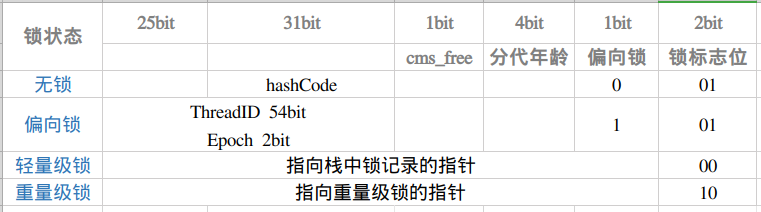
\includegraphics[scale=0.45]{objectheader.png}
	\caption{对象头}
	\label{fig:objectheader}
\end{figure}

https://xiaomi-info.github.io/2020/03/24/synchronized/

\paragraph{轻量级锁(Lightweight Lock)}
引入轻量级锁的主要目的是,在没有多线程竞争的前提下,减少传统的重量级锁使用操作系统互斥量产生的性能消耗(多指时间消耗)。轻量级锁是 JDK1.6 加入的新型锁机制,名字中的「轻量级」是相对于操作系统互斥量这个重量级锁而言的。轻量级锁诞生的原因,是由于对于绝大部分的锁而言,整个同步周期都不存在竞争。如果没有竞争的话,那就没必要使用重量级锁了,于是就诞生了轻量级锁来提高效率。对于轻量级锁来说,其同步的流程如下:

在代码进入同步块的时候,如果此同步对象没有被锁定(锁标志位为 01 状态),那么虚拟机会在当前线程的栈帧中建立一个名为锁记录(Lock Record)的空间,用于存储锁对象目前的 Mark Word 拷贝。

虚拟机将使用 CAS 操作尝试将对象的 Mark Word 更新为指向 Lock Record 的指针。如果更新动作成功了,那么线程就拥有了该对象的锁,并且对象 Mark Word 的锁标志位就变成了 00,表示此对象处于轻量级锁定状态。对应的Hotspot C++代码是:

\begin{lstlisting}[language=C++]
void ObjectSynchronizer::slow_enter(Handle obj, BasicLock* lock, TRAPS) {
    markOop mark = obj->mark();
    assert(!mark->has_bias_pattern(), "should not see bias pattern here");
    
    if (mark->is_neutral()) {
        // Anticipate successful CAS -- the ST of the displaced mark must
        // be visible <= the ST performed by the CAS.
        lock->set_displaced_header(mark);
        if (mark == obj()->cas_set_mark((markOop) lock, mark)) {
        TEVENT(slow_enter: release stacklock);
        return;
        }
        // Fall through to inflate() ...
    } else if (mark->has_locker() &&
                THREAD->is_lock_owned((address)mark->locker())) {
        assert(lock != mark->locker(), "must not re-lock the same lock");
        assert(lock != (BasicLock*)obj->mark(), "don't relock with same BasicLock");
        lock->set_displaced_header(NULL);
        return;
    }
    
    // The object header will never be displaced to this lock,
    // so it does not matter what the value is, except that it
    // must be non-zero to avoid looking like a re-entrant lock,
    // and must not look locked either.
    lock->set_displaced_header(markOopDesc::unused_mark());
    ObjectSynchronizer::inflate(THREAD,
                                obj(),
                                inflate_cause_monitor_enter)->enter(THREAD);
}
\end{lstlisting}

简单地说,轻量级锁的同步流程可以总结为:使用 CAS 操作,在线程栈帧与锁对象建立双向的指针。在没有线程竞争的情况下,轻量级锁使用 CAS 自旋操作避免了使用互斥量的开销,提高了效率。但如果存在锁竞争,除了互斥量的开销外,还额外发生了 CAS 操作。因此在有竞争的情况下,轻量级锁会比传统的重量级锁更慢。

\paragraph{自旋锁(Spin Lock)}所谓自旋锁,就是让该线程等待一段时间,不会被立即挂起,看持有锁的线程是否会很快释放锁。怎么等待呢?执行一段无意义的循环即可(自旋)。自旋发生在Synchronized重量级锁里。
自旋等待不能替代阻塞,虽然它可以避免线程切换带来的开销,但是它占用了处理器的时间。如果持有锁的线程很快就释放了锁,那么自旋的效率就非常好,反之,自旋的线程就会白白消耗掉处理的资源,它不会做任何有意义的工作,这样反而会带来性能上的浪费。所以说,自旋等待的时间(自旋的次数)必须要有一个限度,如果自旋超过了定义的时间仍然没有获取到锁,则应该被挂起。

\paragraph{锁升级Lock Upgrade、锁膨胀Lock Expansion}

https://www.51cto.com/article/713041.html

\end{document}